\documentclass[conference]{IEEEtran}
\IEEEoverridecommandlockouts
\usepackage{cite}
\usepackage{amsmath,amssymb,amsfonts}
\usepackage{algorithmic}
\usepackage{graphicx}
\usepackage{textcomp}
\usepackage{xcolor}
\def\BibTeX{{\rm B\kern-.05em{\sc i\kern-.025em b}\kern-.08em
    T\kern-.1667em\lower.7ex\hbox{E}\kern-.125emX}}
\setlength{\textfloatsep}{8pt plus 2pt minus 4pt}
\setlength{\floatsep}{6pt plus 2pt minus 2pt}
\setlength{\intextsep}{8pt plus 2pt minus 2pt}
\begin{document}

\title{Inspection and Quality Control Robots}

\author{
\IEEEauthorblockN{Veer Sanghvi}
\IEEEauthorblockA{\textit{School of Engineering} \\
\textit{Wentworth Institute of Technology}\\
Boston, MA, USA \\
sanghviv@wit.edu}
\and
\IEEEauthorblockN{Tyler Fong}
\IEEEauthorblockA{\textit{School of Engineering} \\
\textit{Wentworth Institute of Technology}\\
Boston, MA, USA \\
fongt@wit.edu}
\and
\IEEEauthorblockN{Syed Irtiza Ali Shah}
\IEEEauthorblockA{\textit{School of Engineering} \\
\textit{Wentworth Institute of Technology}\\
Boston, MA, USA \\
shahs10@wit.edu}
}

\maketitle

\begin{abstract}
Inspection decides how reliable a finished product actually is, and as manufacturing has scaled up, the tools for doing it have moved from handheld optical gauges to sensor-driven automated systems that can pick out a micro dent in a car body or a damaged kernel on a fast-moving grain line. Human inspectors run into a hard limit: they get tired, they miss things, and they cannot always physically reach complicated geometry, and that gap eventually shows up as field failures, recalls, and rework. Prior work chips away at pieces of this problem instead of solving the whole thing. Fixed-mount vision systems work fine on a flat, well-lit surface but break down once defects or geometry get more varied; mobile platforms cover more ground but add positional uncertainty that hurts measurement accuracy; learning-based methods adapt well but need labeled defect data that is expensive to collect for low-volume parts. This paper proposes an inspection and quality control framework that puts adaptive sensing and kinematic control on one robotic platform rather than treating detection and measurement as separate jobs, so a single six-degree-of-freedom arm can do both surface defect detection and dimensional verification across one workspace. Forward and inverse kinematics for a reference arm are verified in MATLAB against the manufacturer's own rigid-body model, using both a general-purpose numerical solver and a generated closed-form solver, across a reproducible study of over two hundred target poses. All reported errors are solver residuals under an ideal rigid-body model, not measurement accuracy of a physical system. The study also characterizes when and why each solver fails: every non-convergence in the numerical solver traces to a target with no joint-limit-feasible solution, which the closed-form solver certifies directly, while the closed-form solver itself shows one demonstrated false-infeasible verdict caused by floating-point branch loss. These results are used to argue that kinematic feasibility screening belongs in the inspection planner of any manufacturing cell where dimensional and visual inspection still run as separate stations.
\end{abstract}

\textit{Keywords—robotic inspection, quality control automation, defect detection, kinematic modeling, dimensional verification, autonomous manufacturing systems}

\section{Introduction}
Inspection and quality control keeps getting harder as products get more complicated and production cycles get shorter. Manual measurement with calipers and gauges was fine for small production runs, but it could not keep up once volumes grew. Two systems changed that in the late twentieth century: the coordinate measuring machine (CMM), which uses a probe to measure part dimensions precisely, and machine vision, which uses cameras to catch surface defects automatically. Both had a built-in weakness, though. A CMM means pulling the part off the line, and early vision systems were bolted down in one spot, so they could not adjust to a new product or a hidden surface.

Robotic inspection got around that by putting sensors, vision systems, and probes on an arm that can move through the workspace instead of staying still, which is basically a mobile CMM and a mobile vision system combined. These platforms are also starting to feed data analytics pipelines, tracking defect rates and waste over time instead of just flagging one bad part at a time. This paper looks at where robotic inspection stands today, points out where vision-based and contact-based approaches each fall short, and proposes a kinematic and sensing framework meant to close that gap on one platform.

\section{Literature Review}

\subsection{Vision-Based Surface Defect Inspection}
Vision-based detectors make up most of the recent inspection literature, and a lot of the accuracy gains come from adapting the network to the specific defect domain instead of reusing a general-purpose detector off the shelf. Akhyar et al.\ built the Forceful Defect Detector this way, adapting a detection backbone to the low-contrast, irregular texture of steel surface flaws; it beat general-purpose networks on precision, though the authors point out that inference speed and false positives both still matter once the detector has to run on a moving line \cite{ref1}. Zhao et al.\ took a similar approach with RDD-YOLO, building on YOLOv5 with a Res2Net backbone, a double Feature Pyramid Network, and a decoupled detection head, and it beat baseline YOLO variants on both accuracy and recall, especially on small defects (Table \ref{tab:rddyolo}) \cite{ref2}. Bagherzadeh et al.\ went a different direction and surveyed dataset labeling quality instead of model architecture, looking across public benchmarks like NEU-DET and Alibaba's Aluminum Profile Surface Detection Database, and concluded that how consistently the data is labeled matters at least as much as which architecture gets used \cite{ref3}. A 2024 systematic review in \textit{Artificial Intelligence Review} normalized train/test splits across a range of published detection architectures, covering work from 2020 to 2023, and reported a handful of things worth flagging: performance gaps between competing models shrink once the comparison conditions are standardized, supervised detection still dominates the field despite its labeling cost, inspection alone can eat up over half of total manufacturing time in some processes, and dataset imbalance between defective and non-defective samples is still the field's most persistent open problem \cite{ref4}. Chen et al.\ took a different angle from a single camera, pairing a coaxial melt-pool camera, an acoustic microphone, and a thermal camera on a robotic laser-directed energy deposition arm and syncing all three with the arm's motion in time and space, which showed that single-mode vision misses defects that only show up thermally or acoustically \cite{ref5}.

\begin{table}[t]
\caption{RDD-YOLO vs.\ baseline YOLOv5 on steel defect datasets \cite{ref2}}
\label{tab:rddyolo}
\centering
\footnotesize
\setlength{\tabcolsep}{4pt}
\begin{tabular}{lccc}
\hline
Dataset & YOLOv5 mAP & RDD-YOLO mAP & Improvement \\
\hline
NEU-DET & 76.8\% & 81.1\% & +4.3\% \\
GC10-DET & 69.4\% & 75.2\% & +5.8\% \\
\hline
\end{tabular}
\end{table}

\subsection{Modern Inspection and Quality Control Robotic Systems}
Industry 4.0 has pushed artificial intelligence, cloud computing, and machine vision into inspection lines together instead of as separate tools \cite{ref7}\cite{ref8}\cite{ref10}. Six-axis industrial arms carrying cameras, laser scanners, ultrasonic sensors, and CMM probes can run a programmed inspection plan from several angles in a single cycle, and purpose-built platforms like RIPTIDE show the same idea aimed specifically at part inspection rather than general manipulation \cite{ref9}. Collaborative robots extend that same reach into shared workspaces without needing a safety cage \cite{ref13}. Autonomous mobile robots equipped with LiDAR and cameras push inspection even further, like a rail-mounted platform built for concrete quality inspection on aerial building machines \cite{ref11}, patrolling a facility for preventive maintenance and working in places too hazardous to send a person. Sensor fusion, combining cameras, LiDAR, thermal, and ultrasonic data, gives a more complete picture of a part's condition than any one sensor could on its own \cite{ref12}, and letting a robot revise its own inspection program based on what it observes is an active area of research \cite{ref14}. The obstacles that keep showing up are the sheer volume of labeled data deep learning needs and the up-front cost of a full robotic cell, both of which still price out a lot of smaller manufacturers. Where \cite{ref12} fuses multiple sensors on a dedicated metrology platform and \cite{ref13} targets manipulation of metallic surfaces with a purpose-built cobot, the system proposed here differs by folding defect detection and dimensional measurement into the motion plan of one general-purpose arm, so the same kinematic model that positions the camera also positions the laser probe; and unlike the self-revising inspection programs surveyed in \cite{ref14}, viewpoint re-planning here is triggered only by a candidate defect, keeping the baseline cycle deterministic.

\subsection{Force-Controlled and Collaborative Robots for Contact-Based Inspection}
Contact-based inspection is solving a different problem than vision: instead of imaging a surface, a probe actually has to touch it accurately, and in some cases stay in contact with it. ACES is a teleoperated, force-controlled six-degree-of-freedom arm built for inspecting the inside of pipes, and its contact sensor locates each touch point relative to the robot's base frame \cite{ref15}. The system is expensive and hard to control once the pipe geometry includes elbows or branch fittings, according to the authors, but it sets up the geometric idea this project leans on in Section \ref{sec:methodologies}: five contact points, as long as no four of them sit on the same plane, are enough to fully determine a cylinder. A 2025 study in \textit{Cyborg and Bionic Systems} built a robotic ultrasound scanner with an adjustable constant-force end effector, combining a passive spring-like mechanism with active force control to keep the probe in consistent contact with skin \cite{ref16}. A co-robotic mammography system breaks contact scanning into three phases, approach, contact, and a linear scan under proportional-integral-derivative (PID) force control, holding a target contact force while it tracks gentle changes in surface curvature \cite{ref17}. A 2024 paper on automatic contact-based 3D scanning uses an open-loop six-degree-of-freedom arm with a digitizer probe and closed-form inverse kinematics to plan straight-line paths point to point, and it was validated against ASME B89.4.22 with sub-millimeter repeatability \cite{ref18}. Reviews of collaborative robots in quality control describe a sharp shift toward in-process inspection between 2014 and 2023, and tie that shift to the push toward zero-defect manufacturing under Industry 5.0 \cite{ref19}\cite{ref20}. The force-controlled scanners in \cite{ref16} and \cite{ref17} hold a probe against a compliant surface, and the ACES arm \cite{ref15} carries its contact sensor into confined pipe geometry, while the system proposed here inspects rigid manufactured parts in an open cell and can therefore trade continuous contact force control for non-contact laser and depth sensing, which removes the 7 mm class of positional repeatability those systems accept. Against \cite{ref18} and the cobot deployments surveyed in \cite{ref19} and \cite{ref20}, the difference is scope rather than mechanism: those systems perform dimensional capture or generic in-process checks as dedicated tasks, whereas the framework here schedules dimensional measurement and visual defect screening inside one inspection cycle on one arm. Table \ref{tab:litsummary} lays out all the reviewed sources side by side.

\begin{table}[t]
\caption{Summary of reviewed vision- and contact-based approaches}
\label{tab:litsummary}
\centering
\footnotesize
\setlength{\tabcolsep}{3pt}
\begin{tabular}{p{0.08\linewidth}p{0.40\linewidth}p{0.40\linewidth}}
\hline
Ref & Method & Application \\
\hline
\cite{ref1} & Domain-adapted detector backbone & Steel surface defects \\
\cite{ref2} & RDD-YOLO, Res2Net + FPN & Steel surface defects \\
\cite{ref5} & Multisensor digital twin & Robotic laser deposition \\
\cite{ref15} & 6-DOF force-controlled arm, 5-point fit & Pipe interior inspection \\
\cite{ref17} & 3-phase PID force control & Ultrasound scanning \\
\cite{ref18} & Open-loop 6-DOF arm, digitizer probe & Dimensional 3D scanning \\
\hline
\end{tabular}
\end{table}

\section{Significant Methodologies}
\label{sec:methodologies}
Three of the contact-based papers end up anchoring the proposed methodology, mostly because each one relaxes an assumption the other two hold fixed. Reference \cite{ref18} solves inverse kinematics in closed form to drive a touch probe to a contact point. The end effector's pose gets written as a $4\times4$ homogeneous transform, the wrist center gets solved first since the last three joint axes all meet at one point, the first three joint angles fall out of treating the arm like a two-link planar mechanism, and the last three come from the residual rotation matrix once the wrist center is fixed. Tested against a calibrated sphere under ASME B89.4.22, the system hit a 0.036 mm average diameter error, though single-point repeatability got worse with reach, from $\pm$0.0387 mm at 120 mm out to $\pm$0.0712 mm at 500 mm. The main weakness is that it is open loop, so nothing senses the small elastic deflection that happens the instant the probe makes contact.

Reference \cite{ref15} (ACES) asks a narrower geometric question instead: how few contact points does it actually take to describe a cylinder. Touch five points on a cylindrical wall, as long as no four of them are coplanar, and that is enough to solve for the axis direction $\hat a$, an axis point $q$, and the radius $r$, five unknowns pulled out of five point-to-axis distance constraints. The coplanarity condition doubles as a built-in error check, since breaking it means the fit has no unique solution, so any real implementation needs to check the calibration points are not degenerate before trusting whatever comes out.

Reference \cite{ref17} picks up something \cite{ref15} and \cite{ref18} both skip over: a surface that is not rigid. The probe velocity splits into a tangential piece that holds a fixed scan speed and a normal piece driven by a PID law reacting to the gap between measured and target contact force,
\begin{equation}
v = v_\tau \hat\tau + v_n \hat n, \qquad v_n = K_p(F^* - F) + K_i\!\int (F^*-F)\,dt,
\label{eq:force}
\end{equation}
where $v$ is the commanded probe velocity, $v_\tau$ and $v_n$ are its tangential and normal components, $\hat\tau$ and $\hat n$ are the unit tangent and unit normal of the scanned surface, $F$ is the measured contact force, $F^*$ is the force setpoint, and $K_p$ and $K_i$ are the proportional and integral gains. That law held contact force to $5.18 \pm 0.23$ N against a 5 N target across twenty trials, with about 7 mm of positional repeatability, which is too coarse for dimensional work but good enough to keep the probe in stable contact. Table \ref{tab:anchor} lines the three anchor methods up side by side; together they point toward a design that borrows \cite{ref18}'s closed-form kinematics and \cite{ref17}'s tolerance for an imperfect contact surface, but applied to a rigid manufactured part instead of skin.

\begin{table}[t]
\caption{Comparison of anchor contact-based methods}
\label{tab:anchor}
\centering
\footnotesize
\setlength{\tabcolsep}{3pt}
\begin{tabular}{p{0.08\linewidth}p{0.41\linewidth}p{0.39\linewidth}}
\hline
Ref & Result & Limitation \\
\hline
\cite{ref18} & 0.036 mm sphere-fit error, closed-form IK & Open loop, no contact-deflection sensing \\
\cite{ref15} & 5-point cylinder determination & Fails on coplanar points; costly at fittings \\
\cite{ref17} & Force held to $5.18\pm0.23$ N & $\sim$7 mm repeatability, no depth sensing \\
\hline
\end{tabular}
\end{table}

\section{Proposed Methodology}
The proposed system puts a high-definition camera, a depth camera, and a laser displacement sensor on a six-degree-of-freedom robotic arm instead of relying on a fixed inspection station, so the sensor cluster can reach angles a stationary camera never could. A part shows up on the conveyor, trips a proximity sensor, and the arm swings to an initial viewing pose, where a convolutional neural network screens the image for dents, scratches, cracks, missing features, and surface marring. Parts that pass the visual check go straight to dimensional measurement with the laser and depth sensor; parts that trip a possible defect send the arm to a couple more viewpoints first, which cuts down on false positives from shadows or glare before anything actually gets rejected.

The arm's motion follows the Denavit--Hartenberg (DH) convention, so each joint transform is a homogeneous matrix and the tool-frame pose comes out as the product of all six,
\begin{equation}
T_6^0(\mathbf{q}) = A_1(\theta_1)A_2(\theta_2)A_3(\theta_3)A_4(\theta_4)A_5(\theta_5)A_6(\theta_6),
\label{eq:fk}
\end{equation}
with each individual link transform written as
\begin{equation}
A_i = \begin{bmatrix}
c\theta_i & -s\theta_i c\alpha_i & s\theta_i s\alpha_i & a_i c\theta_i \\
s\theta_i & c\theta_i c\alpha_i & -c\theta_i s\alpha_i & a_i s\theta_i \\
0 & s\alpha_i & c\alpha_i & d_i \\
0 & 0 & 0 & 1
\end{bmatrix}.
\label{eq:dh}
\end{equation}
In Eqs.~\eqref{eq:fk} and \eqref{eq:dh}, $\theta_i$, $d_i$, $a_i$, and $\alpha_i$ are the DH joint angle, link offset, link length, and link twist of joint $i$; $c\theta_i$ and $s\theta_i$ abbreviate $\cos\theta_i$ and $\sin\theta_i$, and likewise for $\alpha_i$; $\mathbf{q}=[\theta_1,\ldots,\theta_6]$ collects the six joint angles; and $T_6^0$ is the homogeneous transform of the tool frame expressed in the base frame. Forward kinematics, Eq.~\eqref{eq:fk}, gives the sensor's pose once the joint angles are known; inverse kinematics goes the other way and recovers the joint angles $\mathbf{q}$ needed to put the sensor cluster at some desired inspection pose $T^*$, $\mathbf{q} = f^{-1}(T^*)$. Section \ref{sec:results} applies both to a reference arm and checks them against each other in MATLAB, using a numerical solver and a generated closed-form solver side by side.

The fusion step works as follows. Every CNN detection is a bounding box in image coordinates with a class label and a confidence score. The pixel center of each detection is back-projected through the camera's intrinsic matrix and combined with the depth camera's range value at that pixel, which gives the defect a 3D position in the camera frame; multiplying through the calibrated camera-to-flange transform and the arm's forward kinematics, Eq.~\eqref{eq:fk}, expresses that position in the part's coordinate system. That 3D point becomes the target for re-inspection: the planner requests a pose that puts the laser displacement sensor normal to the surface at the defect location, and inverse kinematics converts it to joint angles, with the feasibility screening of Section \ref{sec:results} deciding whether the pose is reachable before the arm ever moves. At the measurement stage, the laser reading provides a single high-accuracy range sample while the depth camera provides a lower-accuracy patch around it; the two are combined by confidence weighting, with the laser value dominating at its measurement spot and the depth patch supplying surface context around it. The pass/fail decision is a direct comparison of the fused surface deviation against the tolerance band the part's CAD model assigns to that feature: a deviation inside the band passes, one outside it is classified as a defect, and the report recording defect type, location, dimensions, and image evidence gets written to a quality-control database. Comparing the robot's results against a CMM and manual inspection on parts with known defects is how we would find out whether the robotic result is statistically as good as, or better than, the methods it is meant to replace.

\section{Implementation}
The proposed platform is a six-degree-of-freedom industrial arm, something like the ABB IRB 120 or the FANUC LR Mate 200iD. Both are accurate and repeatable enough for precision inspection, and both share the six-revolute, spherical-wrist layout used in Section \ref{sec:results}. A custom bracket holds the camera, depth sensor, and laser displacement sensor at the end effector without dragging down arm performance. A conveyor feeds parts to a proximity sensor that kicks off the inspection cycle, and a programmable logic controller routes accepted parts back to the line and diverts rejects for rework.

CAD models get built in SolidWorks and imported into robot simulation software, FANUC RoboGuide or ABB RobotStudio, for collision checking, reachability analysis, and path optimization before anything gets built physically. MATLAB is what verifies the forward and inverse kinematics and analyzes trajectories, which is exactly what Section \ref{sec:results} does; Python with OpenCV handles image processing, and a convolutional neural network classifies defects. The controller, vision system, and PLC all talk over Ethernet for real-time data exchange. At the software level, the cycle runs: detect part arrival, move to home, move to the inspection pose, capture an image, run defect classification, revisit extra viewpoints if a defect looks likely, take laser and depth measurements, fuse the sensor data, compare against CAD tolerance, sort the part, log the result. The system is built to take on more sensing later, such as ultrasonic or thermal probes, without needing a redesign, so the architecture should outlast whatever sensor choice gets made first.

\section{Results and Analysis}
\label{sec:results}
This section takes the kinematic model from Section \ref{sec:methodologies} and applies it to a reference six-degree-of-freedom arm, verified computationally in MATLAB R2026a with the Robotics System Toolbox. Instead of retyping DH parameters from a secondary source, \texttt{loadrobot('abbIrb120')} pulls a \texttt{rigidBodyTree} built straight from ABB's own kinematic and visual description, so the forward-kinematics chain, joint limits, and inverse-kinematics results below all trace back to that model directly. The ABB IRB 120 got picked because its last three joint axes intersect at a single point, a property the literature relies on to derive closed-form inverse kinematics for this class of arm \cite{ref21}; the FANUC LR Mate 200iD shares that same layout, so the results below should carry over to either candidate from Section \ref{sec:methodologies}. Two solvers run side by side throughout: the toolbox's general-purpose numerical solver (damped least squares on the manipulator Jacobian, random restart enabled) and a closed-form solver generated for this arm by the toolbox's \texttt{analyticalInverseKinematics} tool. Every experiment uses a recorded random seed and archives the full joint vectors, so all results below are reproducible from the published scripts and result files\footnote{Scripts, archived joint vectors, and result CSVs: \texttt{github.com/Veer-Sanghvi/IQCR}.}. Table \ref{tab:dh} lists the equivalent DH parameters for reference against the general form in Eq.~\eqref{eq:dh}.

\begin{table}[t]
\caption{DH parameters, reference six-DOF arm \cite{ref21}}
\label{tab:dh}
\centering
\begin{tabular}{ccccc}
\hline
Link $i$ & $a_i$ (mm) & $\alpha_i$ (deg) & $d_i$ (mm) & $\theta_i$ \\
\hline
1 & 0   & 0   & 290 & var. \\
2 & 270 & -90 & 0   & var. \\
3 & 70  & 0   & 0   & var. \\
4 & 0   & -90 & 302 & var. \\
5 & 0   & 90  & 0   & var. \\
6 & 0   & -90 & 72  & var. \\
\hline
\end{tabular}
\end{table}

One correction from the original submission needs stating up front. The original verification script read joint limits from the first six bodies of the loaded model, but the model's first body is a fixed base link, so that indexing froze the base joint at zero and applied each remaining joint's limits to its neighbor. Targets could therefore be generated from configurations up to a few degrees outside the true joint range. The experiments in Sections \ref{sec:feasible} and \ref{sec:batch} sample each revolute joint's own published limits, and Section \ref{sec:failstudy} deliberately retains the original recipe as a stress test, because it turns out to reproduce, and explain, the non-convergent case reported in the original submission.

\subsection{Verification on feasible targets}
\label{sec:feasible}
Eight target poses were generated by running forward kinematics on joint angles drawn uniformly from within 70\% of each joint's published limits (seed \texttt{rng(7)}), and the numerical solver started from an initial guess perturbed $\pm 7.5^\circ$ per joint away from the true solution. All eight converged, with final position residuals between $2.9\times10^{-7}$ and $3.1\times10^{-5}$~mm in 21--37 iterations (Table \ref{tab:ikresults}). The closed-form solver returned between 2 and 6 joint-limit-feasible solution branches per pose, and its best branch reproduced each target to at or below $2.3\times10^{-12}$~mm, which is machine-precision agreement with the forward-kinematics ground truth.

\begin{table}[t]
\caption{Feasible-target verification, 8 poses, seed \texttt{rng(7)}: numerical solver vs.\ closed-form (CF) branches and best-branch residual}
\label{tab:ikresults}
\centering
\scriptsize
\setlength{\tabcolsep}{2pt}
\begin{tabular}{ccccccc}
\hline
Case & Num.\ (mm) & Ori.\ (deg) & Iter. & Conv. & CF br. & CF (mm) \\
\hline
1 & $3.05\times10^{-5}$ & $1.7\times10^{-6}$ & 21 & yes & 2 & $1.61\times10^{-12}$ \\
2 & $8.30\times10^{-7}$ & 0 & 25 & yes & 4 & $1.84\times10^{-12}$ \\
3 & $6.12\times10^{-7}$ & 0 & 28 & yes & 4 & $2.17\times10^{-12}$ \\
4 & $3.90\times10^{-7}$ & 0 & 34 & yes & 3 & $1.83\times10^{-12}$ \\
5 & $2.43\times10^{-6}$ & 0 & 25 & yes & 2 & $2.15\times10^{-12}$ \\
6 & $2.94\times10^{-7}$ & $1.2\times10^{-6}$ & 37 & yes & 6 & $2.27\times10^{-12}$ \\
7 & $4.19\times10^{-6}$ & $1.2\times10^{-6}$ & 24 & yes & 2 & $1.50\times10^{-12}$ \\
8 & $2.62\times10^{-6}$ & 0 & 25 & yes & 4 & $1.55\times10^{-12}$ \\
\hline
\end{tabular}
\end{table}

\subsection{Batch statistics over 100 random poses}
\label{sec:batch}
To move beyond hand-count sample sizes, 100 additional targets were generated with the same recipe under a second recorded seed (\texttt{rng(11)}). The numerical solver converged on 100 of 100, with a median of 28 iterations, a range of 22 to 214, and a maximum final position residual of $2.1\times10^{-5}$~mm; the single 214-iteration case is one where the solver's random restart engaged and then recovered. The closed-form solver found at least one joint-limit-feasible branch for all 100 targets, with best-branch residuals at or below $1.4\times10^{-10}$~mm. One scope note applies to every convergence statistic in this paper: initial guesses sit within $\pm7.5^\circ$ per joint of a known solution, matching the original protocol, so these results say nothing about convergence from cold starts or distant seeds, and the failure classification in Section \ref{sec:failstudy} is a statement about this initialization regime. Figure \ref{fig:ikiterhist} shows the iteration-count distribution and Figure \ref{fig:ikreshist} the residual distribution across the converged batch.

\begin{figure}[t]
\centering
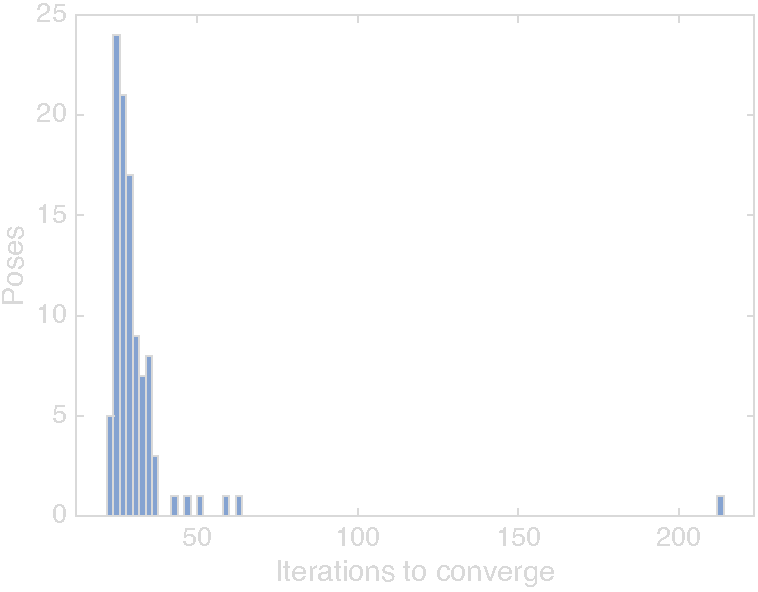
\includegraphics[width=0.85\linewidth]{fig_rst_iter_hist.pdf}
\caption{Iteration counts across the 100-pose batch, seed \texttt{rng(11)}.}
\label{fig:ikiterhist}
\end{figure}

\begin{figure}[t]
\centering
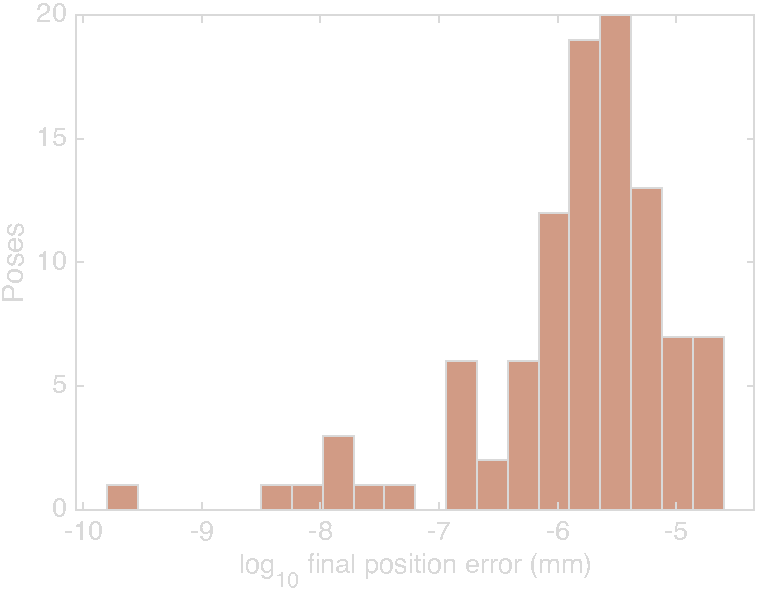
\includegraphics[width=0.85\linewidth]{fig_rst_residual_hist.pdf}
\caption{Distribution of final position residuals ($\log_{10}$, mm) across the 100-pose batch.}
\label{fig:ikreshist}
\end{figure}

\subsection{Failure study: infeasible targets and the original case 8}
\label{sec:failstudy}
The original submission reported one non-convergent pose out of eight: 32.658~mm of position error and $0.111^\circ$ of orientation error after 1500 iterations. The reviewer asked for its root cause, and finding it required reproducing the sampling recipe that generated it. A third experiment therefore ran 100 targets under the original submission's limit indexing (seed \texttt{rng(13)}), the recipe described in the correction note above. Figure \ref{fig:orig8} reproduces the original submission's per-pose chart from its archived results, so the case being analyzed stays visible exactly as it was reported.

The results separate cleanly. Six of the 100 targets were generated from configurations that violate the true joint limits, by margins between $0.13^\circ$ and $6.33^\circ$. The closed-form solver returned zero joint-limit-feasible branches for five of them, certifying those five targets as infeasible, and exactly those five are the poses on which the numerical solver failed to converge. Every failure shows the same signature as the original case 8: the solver runs to its 1500-iteration cap, the orientation error stays below $0.13^\circ$, the position error lands between 0.5 and 30~mm, and the returned configuration sits pinned against a joint limit. In all five failures the pinned joint is the one whose generating value violated its limit, joint 2 at $-110^\circ$ or joint 3 at $+70^\circ$ (Table \ref{tab:failures}). Across these five cases the residual position error also tracks the size of the limit violation, from 0.53~mm at a $0.13^\circ$ violation to 29.7~mm at $6.33^\circ$. Figure \ref{fig:e3residuals} keeps those failures visible the same way the original submission kept its case 8 visible: the five non-convergent cases tower six orders of magnitude above the converged cluster on a log scale instead of disappearing into an average. The full six-joint vectors for the generating configuration, the initial guess, and the returned solution of every case, failed and converged, are archived in the result files. Figure \ref{fig:workspace} plots the five failed targets on the reachable envelope: all five sit inside the position workspace, which rules out workspace exclusion. The failure class the reviewer asked to identify is joint-limit infeasibility: the requested position is reachable, but the full pose has no solution inside the joint range, so the solver presses the offending joint against its stop and stalls. The original case 8 came from this same sampling recipe and carries this same signature, so the analysis classifies it the same way. Its exact joint vectors cannot be recovered because the original run predates joint-vector archiving and the toolbox's random stream is not bit-stable across releases, which is itself the reason every experiment in this revision records seeds and archives joint vectors.

\begin{figure}[t]
\centering
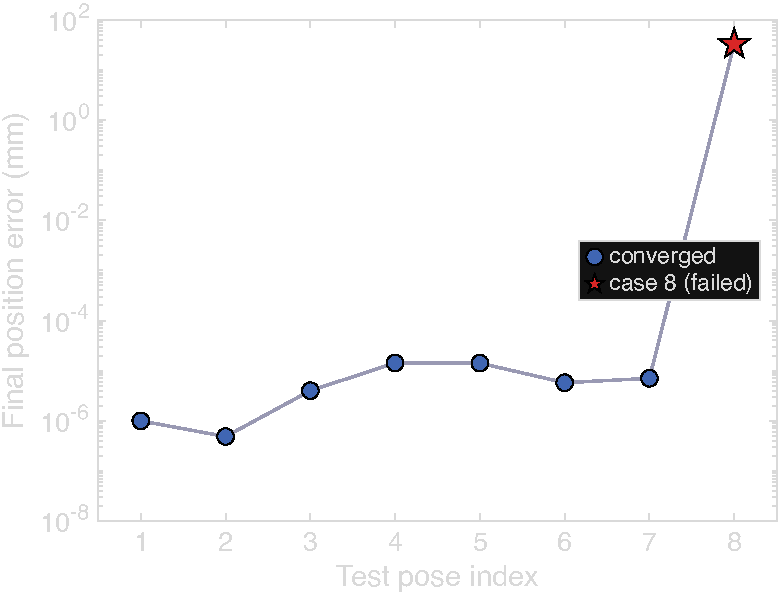
\includegraphics[width=0.85\linewidth]{fig_rst_original8.pdf}
\caption{The original submission's eight-pose run, regenerated as vector graphics from its archived per-case results: seven poses converge to residuals at or below $1.5\times10^{-5}$~mm while case 8 stalls 32.7~mm off target after 1500 iterations.}
\label{fig:orig8}
\end{figure}

\begin{figure}[t]
\centering
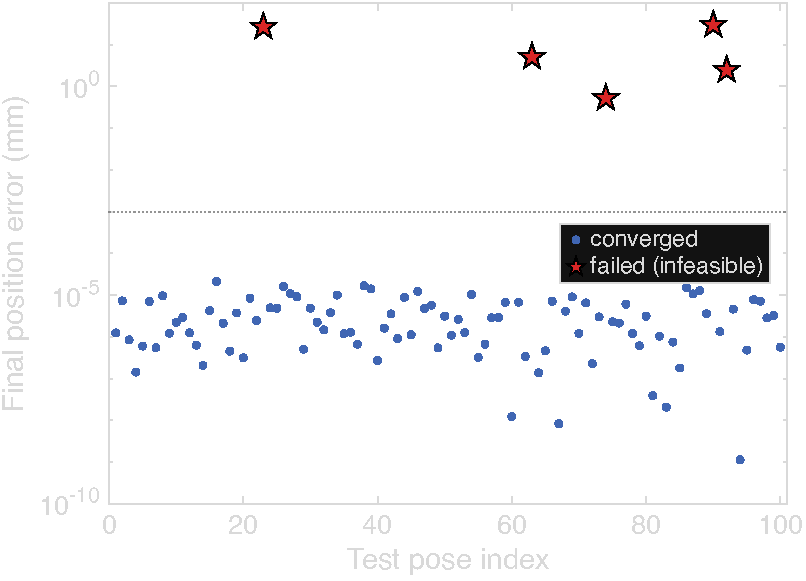
\includegraphics[width=0.85\linewidth]{fig_rst_e3_residuals.pdf}
\caption{Final position error per pose in the infeasible-target study (log scale), seed \texttt{rng(13)}. The five certified-infeasible failures (red stars) stay visible above the converged cluster rather than being averaged away.}
\label{fig:e3residuals}
\end{figure}

\begin{table}[t]
\caption{Failed cases in the infeasible-target study, seed \texttt{rng(13)}}
\label{tab:failures}
\centering
\scriptsize
\setlength{\tabcolsep}{2pt}
\begin{tabular}{cccccc}
\hline
Case & Viol.\ (deg) & Pos.\ err.\ (mm) & Ori.\ err.\ (deg) & CF br. & Pinned joint \\
\hline
23 & 5.67 & 26.69 & 0.046 & 0 & $\theta_3$ at $+70^\circ$ \\
63 & 1.77 & 5.04 & 0.020 & 0 & $\theta_2$ at $-110^\circ$ \\
74 & 0.13 & 0.53 & 0.002 & 0 & $\theta_2$ at $-110^\circ$ \\
90 & 6.33 & 29.68 & 0.121 & 0 & $\theta_3$ at $+70^\circ$ \\
92 & 0.70 & 2.46 & 0.009 & 0 & $\theta_2$ at $-110^\circ$ \\
\hline
\end{tabular}
\end{table}

The sixth zero-branch target is the counterexample. Its generating configuration lies fully inside the true joint limits, and the numerical solver converged on it to $1.4\times10^{-7}$~mm, yet the closed-form solver returned no feasible branch: at full floating-point precision the generated function drops the entire elbow branch family containing the generating configuration, and re-evaluating the same pose after a machine-precision round-trip restores the missing branches. The closed-form verdict is therefore not infallible either; it has a demonstrated false-infeasible failure mode caused by numerical branch loss near an internal tolerance, observed once in this 100-pose study.

\begin{figure}[t]
\centering
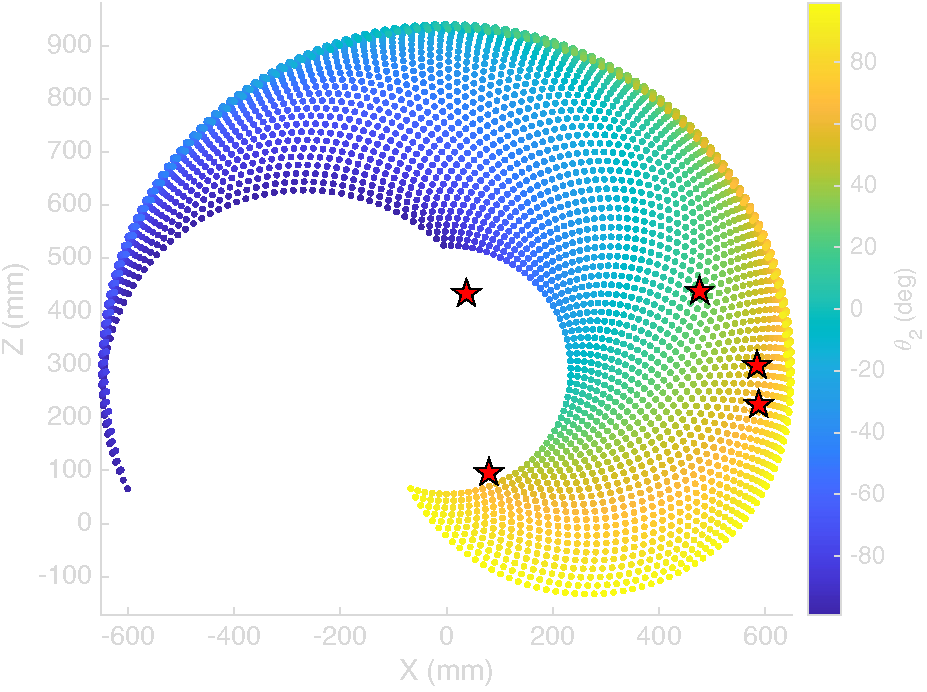
\includegraphics[width=0.85\linewidth]{fig_rst_workspace.pdf}
\caption{Reachable workspace envelope, X--Z plane, base joint fixed at zero, colored by shoulder angle $\theta_2$. Red stars mark the five infeasible targets from Table \ref{tab:failures} at their radial distance from the base axis: all five lie inside the position envelope, so their infeasibility is a joint-limit property of the full pose, not a workspace exclusion.}
\label{fig:workspace}
\end{figure}

Figure \ref{fig:robotpose} renders the loaded model directly at one of the feasible test poses from Table \ref{tab:ikresults}, which confirms the recovered joint angles line up with a physically sensible arm configuration and not just a numerically self-consistent one.

\begin{figure}[t]
\centering
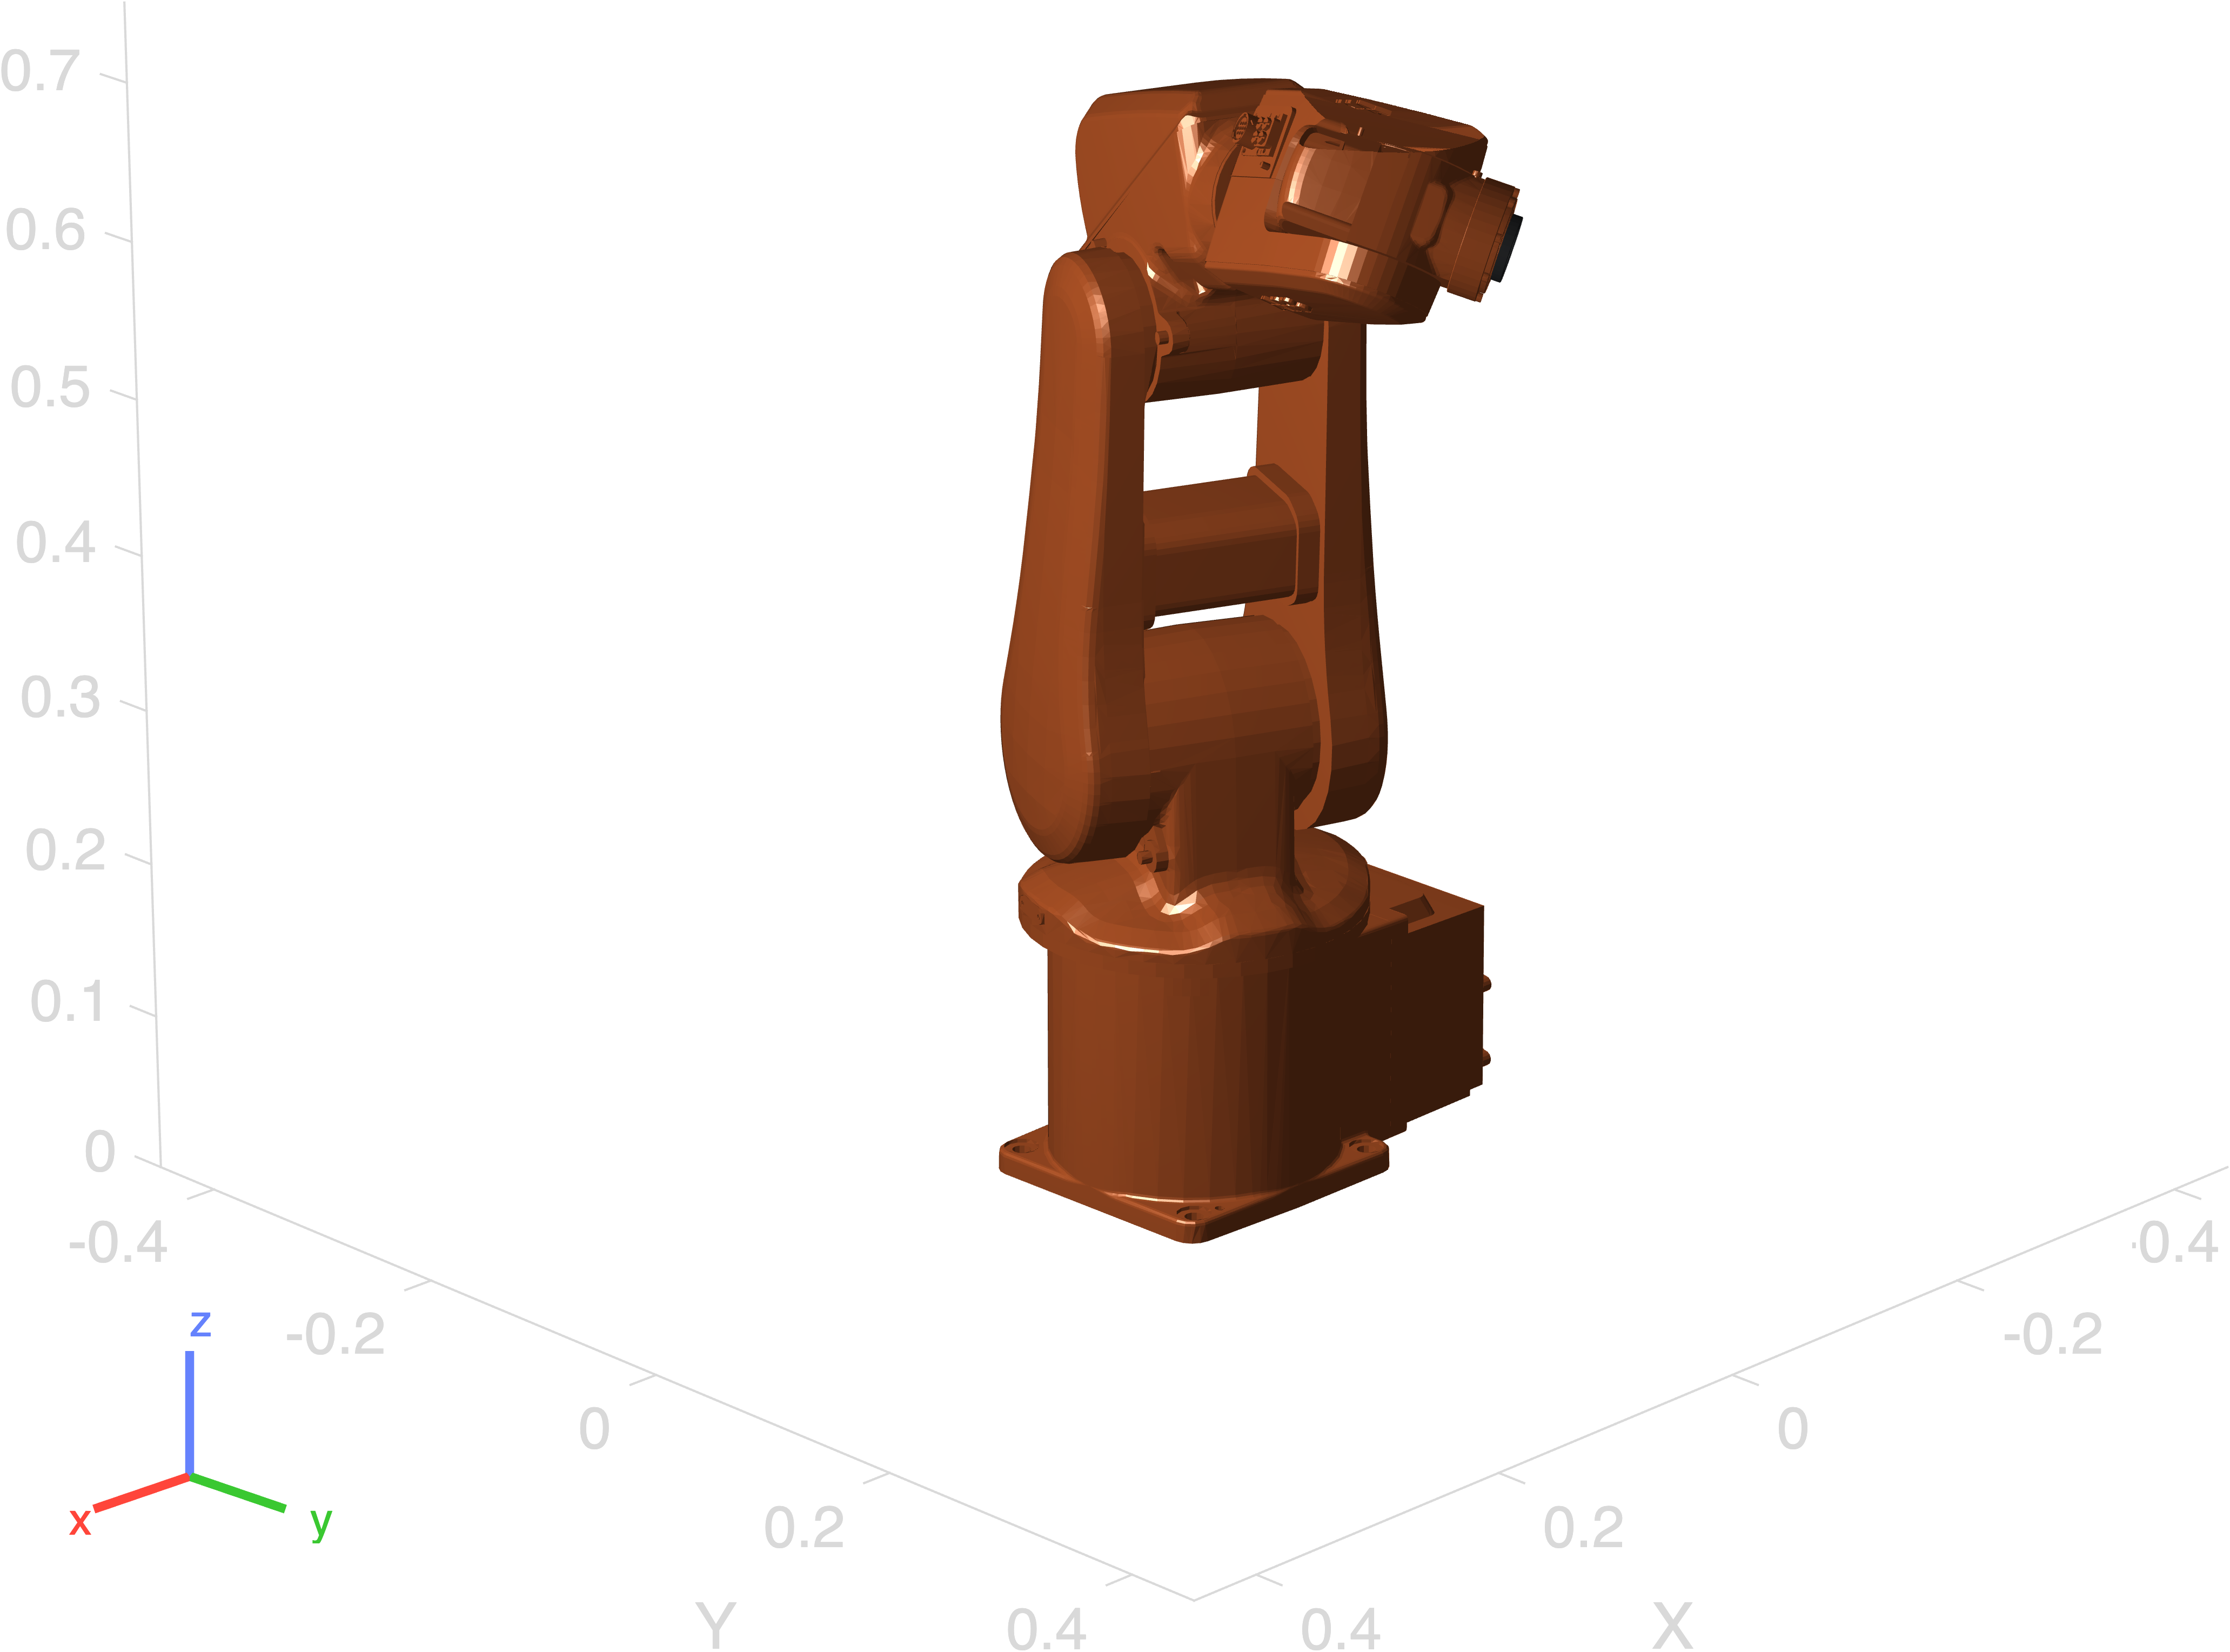
\includegraphics[width=0.62\linewidth]{fig_rst_robot_pose_tight.png}
\caption{Robotics System Toolbox rendering of the reference arm at a feasible test pose.}
\label{fig:robotpose}
\end{figure}


\subsection{Analysis}
Verification here means the loaded model and the solvers agree with each other, and the three experiments back that up from different directions. On feasible targets the numerical solver is reliable and cheap: 108 of 108 convergences across Sections \ref{sec:feasible} and \ref{sec:batch}, a median of 28 iterations, and worst-case residuals five orders of magnitude below any practical inspection tolerance. The closed-form solver reproduces the same targets at machine precision and, more usefully, enumerates every joint-limit-feasible branch, which a local iterative search cannot do.

The failure study is where running both solvers pays off. A numerical solver that hits its iteration cap reports only that it failed, and an inspection cell cannot tell from that report whether the pose was unreachable, blocked by a joint limit, or simply a bad initial guess. The closed-form solver answers that question by construction, because enumerating all branches and finding none inside the joint limits is a certificate of infeasibility rather than a failed search. In this study that certificate was correct for all five numerical failures. The converse case matters just as much: one feasible pose lost its entire elbow branch family to floating-point sensitivity inside the generated closed-form function, producing a false infeasible verdict on a target the numerical solver handled without trouble. Neither solver is sufficient alone. The architecture this points to for a production controller runs the closed-form solver first, for a fast feasibility verdict and a set of branch solutions to seed from, falls back to the numerical solver for refinement, and treats disagreement between the two, closed-form empty but numerical converging, as a flag for the tolerance-boundary case rather than trusting either verdict blindly.

The practical takeaway for the proposed inspection cell is that kinematic feasibility screening needs to happen at planning time, not at execution time. The five certified-infeasible targets in Section \ref{sec:failstudy} are exactly the kind of pose an inspection planner could request after back-projecting a defect detection into a re-inspection viewpoint. Wall-clock cost makes the screening argument concrete: on an Apple M-series laptop CPU, a converged numerical solve takes a median of 4.0~ms, a stalled 1500-iteration solve takes 0.11~s and returns no diagnosis, and one closed-form call takes 0.38~ms. Screening every candidate viewpoint with the closed-form solver therefore costs an order of magnitude less than a single successful numerical solve, and roughly 300 times less than discovering one infeasible request the hard way. The near-proportional relationship between limit violation and residual position error also gives an operator a usable diagnostic: a stalled solve that ends pinned at a joint limit with millimeters of residual points at an infeasible request, not at a solver bug.

The limits of these results need stating plainly. Every error figure in this section is a solver residual computed under an ideal rigid-body model: rigid links, ideal revolute joints, exact encoder readings, an exact tool-frame calibration, and no thermal effects. These numbers say nothing about the measurement accuracy of a physical inspection cell. A real arm adds gearbox backlash, joint compliance, encoder quantization, tool-center-point calibration error, thermal drift, and fixturing error on top of everything reported here, and each of those terms is orders of magnitude larger than the solver residuals in Table \ref{tab:ikresults}. No measurement-accuracy claim for the proposed system can be made until the framework is validated on hardware against a coordinate measuring machine, as Section \ref{sec:methodologies} describes.

\section{Conclusion}
This project looked at the shift away from manual and fixed-station inspection and toward robotic inspection and quality control, and proposed a framework that puts vision-based defect detection and dimensional verification on the same six-degree-of-freedom platform instead of splitting them across two systems. Forward and inverse kinematics for a representative reference arm got verified in MATLAB R2026a using the Robotics System Toolbox's own rigid-body-tree model of the ABB IRB 120, with a numerical and a generated closed-form solver run side by side across 208 seeded, reproducible target poses. On feasible targets the numerical solver converged 108 times out of 108 with solver residuals no worse than $3.1\times10^{-5}$~mm against the forward-kinematics ground truth, and the closed-form solver reproduced the same targets at machine precision while enumerating every joint-limit-feasible branch. The failure study explained the non-convergent case from the original submission: targets generated without joint-limit feasibility checking can demand poses no in-limit configuration reaches, the numerical solver responds by pinning a joint against its stop and stalling at its iteration cap, and the closed-form solver certifies the infeasibility directly, while carrying a demonstrated false-infeasible failure mode of its own, observed once in the 100-pose study. These residuals are rigid-body model agreement, not measurement accuracy, and the reachable workspace forms a distorted ring that comfortably covers a small-to-mid-size manufactured part from multiple angles. Combined with the sensor-fusion pipeline proposed in Section \ref{sec:methodologies}, this backs up the paper's central argument, that adaptive sensing and kinematic control belong on one platform with feasibility screening in the planner, while leaving physical validation against a coordinate measuring machine as the necessary step before any accuracy claim about the system itself.

\section{Recommendations}
The first priority is building an actual physical work cell instead of continuing to lean on kinematic simulation alone, since only hardware testing will show how much gearbox backlash, joint compliance, encoder quantization, tool-center-point calibration error, thermal drift, and fixturing error add on top of the solver residuals reported in Table \ref{tab:ikresults}; validation against a coordinate measuring machine on parts with known defects is the concrete test. The dual-solver architecture from Section \ref{sec:results}, closed-form first for a feasibility certificate and branch seeds, numerical refinement second, and solver disagreement flagged rather than trusted, should be implemented on the real controller, along with feasibility screening of every planner-requested viewpoint before motion starts. The single false-infeasible verdict the closed-form solver produced deserves its own follow-up, since characterizing how often generated analytical solvers lose solution branches near internal tolerances matters to anyone using them as a feasibility oracle. The defect-detection network needs a bigger, more varied training set, covering different lighting conditions, materials, and defect types, since detector performance tracks labeled data quality about as consistently as anything in this field, which \cite{ref3} and \cite{ref4} both point out. Later versions should add ultrasonic or thermal sensing to catch internal defects that optical inspection just cannot see, and hook the system into an Industry 4.0 manufacturing stack so inspection data actually feeds predictive maintenance and process optimization instead of sitting in a log nobody looks at.

\section*{Acknowledgment}
This research received no external funding. During the preparation of this work, the author(s) used Claude (Anthropic) to assist with proofreading and checking the validity of reported data and calculations. After using this tool, the author(s) reviewed and edited the content as needed and take full responsibility for the content of the publication.

\IEEEtriggeratref{6}
\begin{thebibliography}{00}
\bibitem{ref1} F. Akhyar, Y. Liu, C.-Y. Hsu, T. K. Shih, and C.-Y. Lin, ``FDD: a deep learning-based steel defect detector,'' \textit{Int. J. Adv. Manuf. Technol.}, vol. 126, no. 3, pp. 1093--1107, 2023.
\bibitem{ref2} C. Zhao, X. Shu, X. Yan, X. Zuo, and F. Zhu, ``RDD-YOLO: A modified YOLO for detection of steel surface defects,'' \textit{Measurement}, vol. 214, p. 112776, 2023.
\bibitem{ref3} F. Bagherzadeh, T. Shafighfard, R. M. A. Khan, P. Szczuko, and M. Mieloszyk, et al., ``A systematic review of deep learning approaches for surface defect detection in industrial applications,'' \textit{Eng. Appl. Artif. Intell.}, 2023.
\bibitem{ref4} Y. Ma et al., ``Surface defect inspection of industrial products with object detection deep networks: a systematic review,'' \textit{Artif. Intell. Rev.}, 2024.
\bibitem{ref5} L. Chen, G. Bi, X. Yao, C. Tan, J. Su, N. P. H. Ng, Y. Chew, K. Liu, and S. K. Moon, ``Multisensor fusion-based digital twin for localized quality prediction in robotic laser-directed energy deposition,'' \textit{Robot. Comput.-Integr. Manuf.}, vol. 84, p. 102581, 2023.
\bibitem{ref7} K. G. Amin, M. Patidar, P. K. Patidar, N. K. R. Rafaliya, J. Joshi, and D. Mishra, ``A review on robotics and automation techniques for quality inspection in Industry 4.0,'' in \textit{2025 IEEE Int. Conf. Adv. Comput. Res. Sci. Eng. Technol. (ACROSET)}, Indore, India, 2025, pp. 1--5.
\bibitem{ref8} A. Villalonga, Y. J. Cruz, D. Alfaro, R. E. Haber, J. L. Mart\'inez-Lastra, and F. Casta\~no, ``Enhancing quality inspection in zero-defect manufacturing through robotic-machine collaboration,'' in \textit{2024 7th Iberian Robotics Conf. (ROBOT)}, Madrid, Spain, 2024, pp. 1--6.
\bibitem{ref9} A. E. Duron, B. A. C. Stiles, and D. A. Torck, ``RIPTIDE: Robot inspecting parts to increase development efficiency,'' in \textit{2025 22nd Int. Conf. Ubiquitous Robots (UR)}, College Station, TX, USA, 2025, pp. 333--339.
\bibitem{ref10} T. Brito, J. Queiroz, L. Piardi, L. A. Fernandes, J. Lima, and P. Leit\~ao, ``A machine learning approach for collaborative robot smart manufacturing inspection for quality control systems,'' \textit{Procedia Manuf.}, vol. 51, pp. 11--18, 2020.
\bibitem{ref11} M. Zhou, C. Ge, and X. Xiong, ``Research on a rail-mounted concrete quality inspection robot system for aerial building machine,'' in \textit{2025 10th Int. Conf. Autom. Control Robot. Eng. (CACRE)}, 2025, pp. 9--16.
\bibitem{ref12} S. Discepolo and P. Castellini, ``Neural network to retrieve features of a mechanical component acquired by a robotic inspection system,'' in \textit{2024 IEEE Int. Conf. Metrology for Extended Reality, Artif. Intell. Neural Eng. (MetroXRAINE)}, 2024, pp. 325--330.
\bibitem{ref13} T. Czimmermann, M. Chiurazzi, M. Milazzo, S. Roccella, M. Barbieri, P. Dario, C. M. Oddo, and G. Ciuti, ``An autonomous robotic platform for manipulation and inspection of metallic surfaces in Industry 4.0,'' \textit{IEEE Trans. Autom. Sci. Eng.}, vol. 19, no. 3, pp. 1691--1706, 2022.
\bibitem{ref14} D. Irvine and M. Narayanan, ``Inspection and quality control - an overview,'' in \textit{IEEE Tech. Appl. Conf. Workshops (Northcon/95)}, 1995, pp. 376--380.
\bibitem{ref15} ``ACES: A teleoperated robotic solution to pipe inspection from the inside,'' arXiv:2405.09925, 2024.
\bibitem{ref16} Z. Wu et al., ``Robotic ultrasound scanning end-effector with adjustable constant contact force,'' \textit{Cyborg Bionic Syst.}, 2025.
\bibitem{ref17} ``Enabling mammography with co-robotic ultrasound,'' arXiv:2312.10309, 2023.
\bibitem{ref18} ``Automatic contact-based 3D scanning using articulated robotic arm,'' presented at Int. Conf. Interactive Design Manuf., 2024.
\bibitem{ref19} ``Collaborative robots for quality control: an overview of recent studies and emerging trends,'' \textit{J. Intell. Manuf.}, 2025.
\bibitem{ref20} M. Al-Amin, ``Cobotics: the evolving roles and prospects of next-generation collaborative robots in Industry 5.0,'' \textit{J. Robot.}, vol. 2024, Art. no. 2918089, 2024.
\bibitem{ref21} O. F. Seven and A. Ankarali, ``Inverse kinematic analysis of IRB120 robot arm,'' \textit{SETSCI Conf. Proc.}, vol. 4, no. 1, pp. 383--390, ISAS2019, Ankara, Turkey, 2019.
\end{thebibliography}

\end{document}
